% dimred

\begin{frame}
  \frametitle{Unsupervised Learning}
  \begin{itemize}
    \item Unlabeled data: 
    \item[] $n$ observations $\{\xvec_1, \xvec_2, \dots, \xvec_n\}$; $\xvec_i \in \xcal = \RR^p$
    \item Objectives: 
    \begin{itemize}
      \item Data exploration
      \item Identification of trends and groups
    \end{itemize} 
    \item Prediction tasks: 
    \begin{itemize}
        \item \red{Dimensionality reduction:} $f : \RR^p \rightarrow \RR^d$ with
          $d \ll p$, such that $f(\xvec)$ is an
          \blue{informative representation} of $\xvec$
        \item \red{Clustering:} partitioning $\{1, 2, \dots, n\}$ into sets
        of similar elements, called \red{clusters}
    \end{itemize}
    \item Note: dimensionality reduction can be either supervised or unsupervised. 
    \end{itemize}
\end{frame}

\begin{frame}
  \begin{center}
    \red{\LARGE Dimensionality Reduction}
  \end{center}
\end{frame}

\begin{frame}
  \frametitle{Dimensionality Reduction — Problem}
  \begin{itemize}
  \item Large number $p$ of variables (hundreds or thousands of features).
  \item If $n$ is large, we speak of \red{big data}.   
  \item If $p$ is large compared to $n$, we speak of \red{fat data}. 
  \item Dimensionality reduction: find, for a data matrix $X\in \RR^{n\times p}$, a representation $X' \in \RR^{n\times m}$ with $p \gg m$. 
  \end{itemize}
\end{frame}

\begin{frame}
  \frametitle{Dimensionality Reduction — Motivation}
  \begin{itemize}
  \item Visualization / exploration: an essential step
  \item Identify artifacts
  \item Reduce computational cost
  \item Fewer descriptors for better predictive algorithms: 
  \begin{itemize}
    \item fewer parameters to estimate
    \item less noise
    \item fewer non-informative dimensions
    \item avoid the curse of dimensionality
  \end{itemize}
  \end{itemize}
\end{frame}

\begin{frame}
  \frametitle{Dimensionality Reduction — Two Strategies}
  \begin{itemize}
    \item \red{Feature selection:} eliminate variables that are not useful
    \item \red{Feature extraction:} create $m$ new variables from the $p$ original ones
  \end{itemize}
\end{frame}

\begin{frame}
  \frametitle{Filter Methods}
  \begin{itemize}
    \item Unsupervised filtering (e.g., removing correlated variables)
    \item Supervised filtering: removing variables that are not statistically associated with the output variable
  \end{itemize}
\end{frame}

\begin{frame}
  \frametitle{Filter Methods — Limitations}
  \begin{figure}[htb]
    \centering
    
\includegraphics[width=.6\textwidth]{guyon.pdf}
  \end{figure}
    Correlated and individually non-significant variables may still be useful (in the context of other variables).
\end{frame}

\begin{frame}
  \frametitle{Wrapper Methods}
  \begin{itemize}
    \item \red{Supervised} feature selection methods. 
    \item Linked to a \red{classification} method: the quality of a variable is judged based on its effect on classification performance.
    \item Two strategies: 
    \begin{itemize}
      \item \red{Forward selection:} successively add variables
      \item \red{Backward elimination:} successively remove variables
    \end{itemize}
  \end{itemize}
\end{frame}

\begin{frame}
  \frametitle{Forward Selection}
  \begin{itemize}
    \item Start with an empty set of variables $\fcal = \emptyset$
    \item At each step, add the variable that yields the greatest improvement in classification performance.
    \item Stop when performance no longer improves. 
  \end{itemize}
\end{frame}

\begin{frame}
  \frametitle{Backward Elimination}
  \begin{itemize}
    \item Start with the full set of variables $\fcal$
    \item At each step, remove the variable whose removal gives the best classification performance.
    \item Stop when performance no longer improves. 
  \end{itemize}
\end{frame}

\begin{frame}
  \frametitle{Wrapper Methods — Limitations}
  \begin{itemize}
    \item The selected set of variables depends on the classifier used (it is not a general criterion). 
    \item Greedy method: no guarantee of optimality. 
  \end{itemize}
\end{frame}

\begin{frame}
  \frametitle{Embedded Methods}
  \begin{itemize}
    \item Classification methods that include an integrated variable selection mechanism.
    \item Example: the use of the $L_1$ norm (absolute value).  
    \item Reminder:
  \end{itemize}
  \begin{center}
    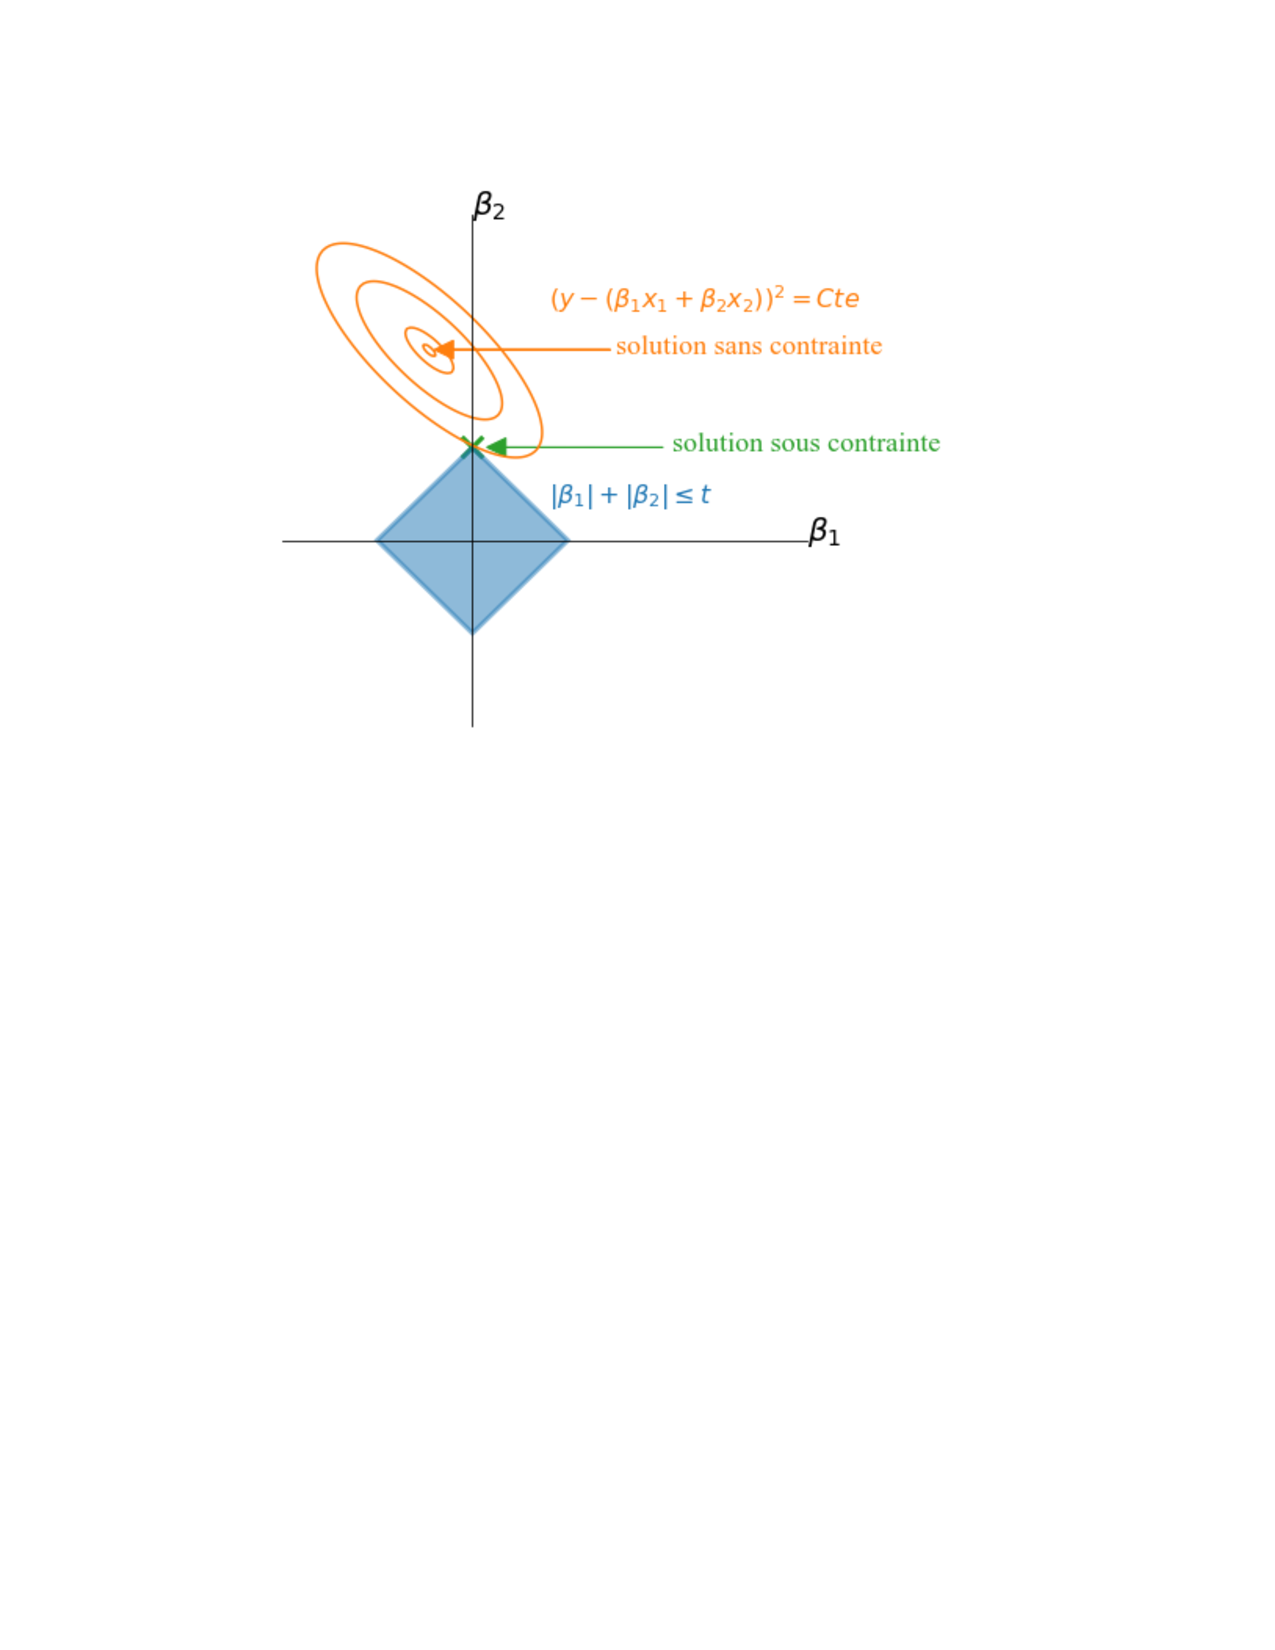
\includegraphics[width=.6\textwidth]{figures/l1reg_geom}  
  \end{center}
\end{frame}

\begin{frame}
  \frametitle{Principal Component Analysis}
  \begin{itemize}
    \item Principal Component Analysis (PCA)
    \item \red{Unsupervised} method (no labels are used)
    \item Expresses $X\in \RR^{n\times p}$ in an orthonormal basis through an orthogonal linear transformation.
    \item Maximizes variance.
%   \item First axis: projection of $X$ with the largest variance
%   \item Second axis: projection of $X$ with the largest variance, orthogonal to the first one.
%   \item $\ldots$
  \end{itemize}
\end{frame}

\begin{frame}
  \frametitle{Feature Extraction — PCA}
  \begin{figure}[htb]
    \centering
    
\includegraphics[width=.8\textwidth]{pca.pdf}
  \end{figure}
\end{frame}

\begin{frame}
\frametitle{PCA: Method 1/3}
  \begin{itemize}
    \item First step: center the columns of $X \in \RR^{n \times p}$:
 \begin{equation*}
 x^i_j = \frac{x_j^i - \overline{x}_j}{\sqrt{\frac{1}{n}\sum_{l=1}^n(x_j^l - \overline{x}_j)^2}} 
 \end{equation*}
  \item Covariance matrix (if $X$ is standardized): $\Sigma = \frac1n X^TX$ 
  \item We seek a direction $\wvec$ such that the projection of $X$ onto this direction has maximal variance. 
  \item It can be shown that this maximum variance corresponds to the largest eigenvalue of $\Sigma$, and that the direction is the corresponding eigenvector. 
  \end{itemize}
\end{frame}

\begin{frame}
\frametitle{PCA: Method 2/3}
  \begin{itemize}
    \item If we order the eigenvalues of $\Sigma$, we obtain the principal components $pc_1, pc_2, \ldots$ which satisfy the following criteria: 
    \begin{itemize}
      \item Each $pc_i$ is orthogonal to all other components.
      \item The variance of the projection of $X$ on $pc_i$ equals the $i$-th eigenvalue. 
    \end{itemize}
    \item We can deduce that: 
    \begin{itemize}
      \item The projections of $X$ onto the principal components are uncorrelated. 
      \item The principal components $pc_i$ contain decreasing amounts of information as $i$ increases. 
    \end{itemize}
  \end{itemize}
\end{frame}

\begin{frame}
\frametitle{PCA: Method 3/3}
  \begin{itemize}
    \item PCA thus provides a transformation yielding variables that are uncorrelated and ordered according to their variance, which is assumed to reflect their information content. 
    \item Typically, we select a number $m$ of principal components. The criterion for $m$ is the “explained” variance of the model:
    \begin{equation}
      \frac{\sum_{j=1}^{m}var(X\wvec_j)}{\sum_{j=1}^pvar(X\wvec_j)}
    \end{equation}
    \item Alternatively, one may choose $m=2$ or $m=3$ for visualization purposes.   
  \end{itemize}
\end{frame}

\begin{frame}
\frametitle{PCA: Advantages and Limitations}
  \begin{itemize}
    \item Advantages: 
    \begin{itemize}
      \item Unsupervised
      \item Uncorrelated projections 
      \item Simple linear method
    \end{itemize}
    \item Limitations: 
    \begin{itemize}
      \item Maximal variance does not necessarily correspond to maximal information content
      \item In practice, local structures are not always well preserved 
    \end{itemize}
  \end{itemize}
\end{frame}

\begin{frame}
\frametitle{t-SNE 1/3}
\begin{itemize}
% \item Many low-dimensional representations: PCA, ICA, $\ldots$
  \item Objective: obtain a low-dimensional representation of the data while preserving local relationships.
  \item A relatively recent technique — \emph{t-Distributed Stochastic Neighbor Embedding (t-SNE)} (2008)
  \item $\{\xvec_i\}_{0\leq i < N}$ are the data points, with $\xvec_i \in \RR^p$. 
  \item We define the probability that $\xvec_j$ is a neighbor of $\xvec_i$, assuming that this probability can be modeled by a Gaussian centered at $\xvec_i$:  
  \begin{equation}
  p_{j|i} = \frac{\exp{\left(-\frac{\|\xvec_i - \xvec_j\|^2}{2 \sigma_i^2}\right)}}{\sum_{k\neq i} \exp{\left(-\frac{\|\xvec_i - \xvec_k\|^2}{2 \sigma_i^2}\right)} }
  \end{equation}
  The parameter $\sigma_i$ varies with each sample $x_i$. 
\end{itemize}
\end{frame}

\begin{frame}
\frametitle{t-SNE 2/3}
\begin{itemize}
  \item We aim to assign the vectors $\{\xvec_i\}$ new representations $\{\widetilde{\xvec_i}\}$ while preserving the neighborhood probabilities $q_{j|i}$: 
  \begin{equation*}
  q_{j|i} = \frac{\exp{\left(-\|\widetilde{\xvec_i} - \widetilde{\xvec_j}\|^2\right)}}{\sum_{k\neq i} \exp{\left(-\|\widetilde{\xvec_i} - \widetilde{\xvec_k}\|^2\right)} }
  \end{equation*}
  \item This is achieved by minimizing the Kullback–Leibler divergence between the distributions $P_i$ (distribution of $p_{j|i}$) and $Q_i$ (distribution of $q_{j|i}$): 
  \begin{equation}
    C = \sum_i KL(P_i\|Q_i) = \sum_i \sum_j p_{j|i}\log{\frac{p_{j|i}}{q_{j|i}}}
  \end{equation}
  \item If $\xvec_i$ and $\xvec_j$ are close in the original space, the algorithm tries to push $q_{j|i}$ toward $p_{j|i}$ (so that the ratio approaches 1). 
  \item If $\xvec_i$ and $\xvec_j$ are far apart in the original space, this is not guaranteed in the low-dimensional space. 
\end{itemize}
\end{frame}

\begin{frame}
\frametitle{t-SNE 3/3}
\begin{itemize}
  \item The parameters $\sigma_i$ are determined automatically by the algorithm.
  \item They vary depending on the local density of neighbors, such that each $\xvec_i$ has approximately the same number of neighbors. 
  \item The user chooses the \textit{perplexity} parameter, which measures the effective number of neighbors. 
  \item The problem is then reduced to solving an optimization problem $\min_{\widetilde{\xvec_i}} C$ using gradient descent.
\end{itemize}
\end{frame}

\begin{frame}
\frametitle{t-SNE: Advantages and Limitations}
  \begin{itemize}
    \item Advantages: 
    \begin{itemize}
      \item Preserves local structures
      \item Helps identify potential clusters 
    \end{itemize}
    \item Limitations: 
    \begin{itemize}
      \item No transformation: the minimization is performed on a given dataset and cannot be directly applied to new data 
      \item Distortion of long-range distances 
    \end{itemize}
  \end{itemize}
\end{frame}

\begin{frame}
\frametitle{Example of a t-SNE Map: ImageNet}
\begin{itemize}
  \item In modern Computer Vision, images are mapped to vectors $\xvec \in \RR^p$, with $p$ typically in the hundreds or thousands. 
  \item These vectors are then further processed (for instance classification)
  \item Here, we will investigate the vector representations $\{\xvec_i\}_{i = 1..N}$ of a subset of the ImageNet dataset (a large set of natural images). 
\end{itemize}
\end{frame}


\begin{frame}
\frametitle{t-SNE Map: ImageNet}
\begin{figure}[htb]
  \centering
  
\includegraphics[width=\textwidth]{Vis_tsne_imagenet1.pdf}
%  \source{adapted from \url{https://cs.stanford.edu/people/karpathy/cnnembed/}}
\end{figure}
\end{frame}

\begin{frame}
\frametitle{t-SNE Map: ImageNet}
\begin{figure}[htb]
  \centering
  
\includegraphics[width=\textwidth]{Vis_tsne_imagenet2.pdf}
%  \source{adapted from \url{https://cs.stanford.edu/people/karpathy/cnnembed/}}
\end{figure}
\end{frame}

\begin{frame}
\frametitle{t-SNE Map: ImageNet}
\begin{figure}[htb]
  \centering
  
\includegraphics[width=\textwidth]{Vis_tsne_imagenet3.pdf}
%  \source{adapted from \url{https://cs.stanford.edu/people/karpathy/cnnembed/}}
\end{figure}
\end{frame}

\begin{frame}
\frametitle{Conclusion}
\begin{itemize}
  \item Ad-hoc filtering methods
  \item Wrapper methods: variable selection for a specific classification task
  \item Embedded methods (e.g. LASSO)
  \item PCA: principal component analysis
  \item t-SNE: a method used primarily for visualization
\end{itemize}
\end{frame}

\begin{frame}
  \begin{center}
    \red{\LARGE Clustering} 
  \end{center}
\end{frame}

\begin{frame}
  \frametitle{Clustering or Partitioning}
  \begin{itemize}
  \item \red{Clustering:} partitioning data into homogeneous subsets (\red{clusters})
  \item Examples:
    \begin{itemize}
    \item \blue{Market segmentation}
    \item \blue{Communities} in a social network
    \item \blue{Topic modeling} (text thematics)
    \item \blue{Image compression} or \blue{image segmentation}
    \item \blue{Subtypes} of a disease
  \end{itemize}
  \end{itemize}
\end{frame}

\begin{frame}
  \frametitle{Clustering — Motivation}
  \begin{itemize}
  \item Study of \blue{unlabeled} data
  \item \blue{Exploratory} data analysis
  \item \blue{Visualization}
  \item May precede an \blue{inference} phase (e.g., topic modeling)
  \end{itemize}
\end{frame}

\begin{frame}
  \begin{center}
    \large{1. Evaluating a Clustering}
  \end{center}
\end{frame}

\begin{frame}
\frametitle{1.1 Geometric Criteria}
  \begin{center}
    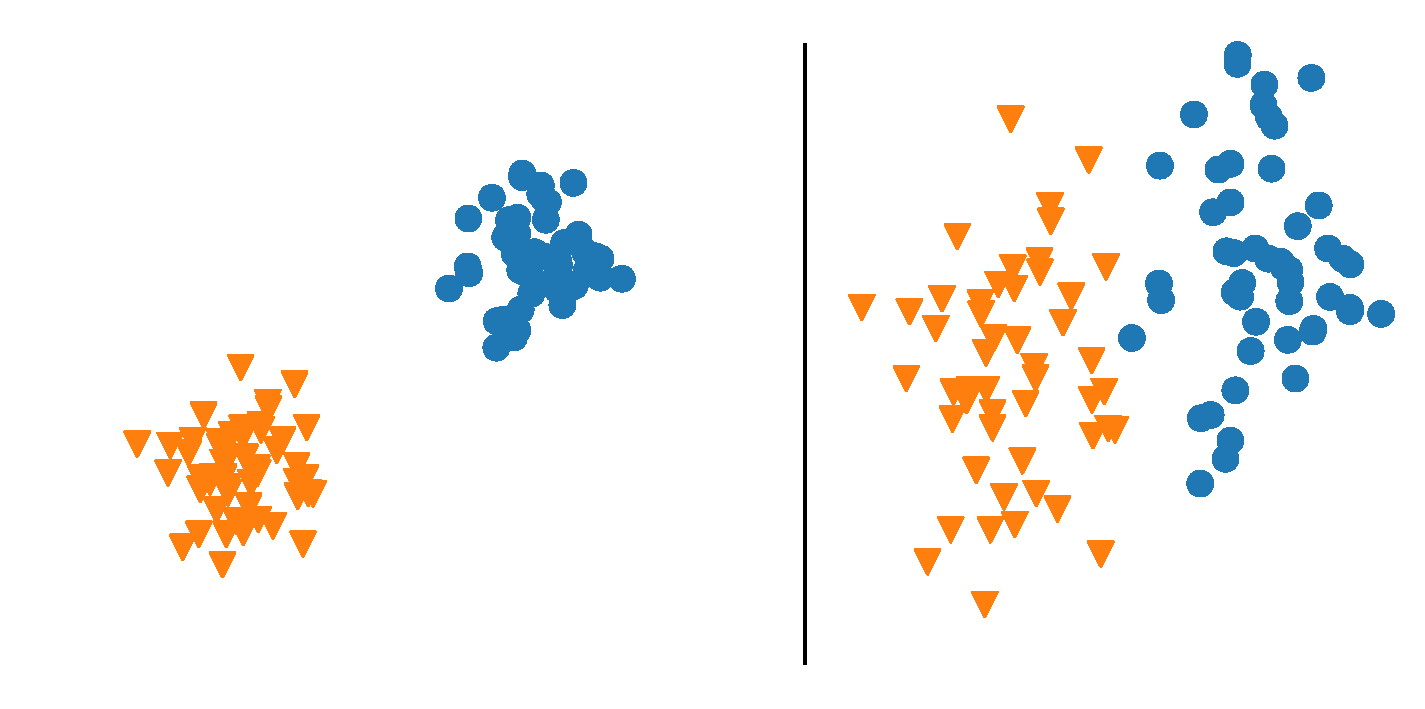
\includegraphics[width=0.5\textwidth]{figures/homogeneity}%
  \end{center}
\begin{itemize}  
  \item Centroid of cluster $\cset$: $\muvec_{\cset} = \frac{1}{|\cset|}\sum_{\xvec \in \cset}\xvec$
  \item Medoid of cluster $\cset$: $\mvec_{\cset} = \argmin_{\xvec \in \cset} d(\xvec, \muvec_{\cset})$
  \item \red{Homogeneity} of a cluster $k$: $T_k = \frac{1}{|\cset_k|} \sum_{\xvec \in \cset_k} d(\xvec, \muvec_k)$
  \item Homogeneity of a clustering:
  \begin{equation*}
  T = \frac1K\sum_{k=1}^{K}T_k
  \end{equation*}
\end{itemize}
\end{frame}

\begin{frame}
\frametitle{1.1 Geometric Criteria}
  \begin{center}
    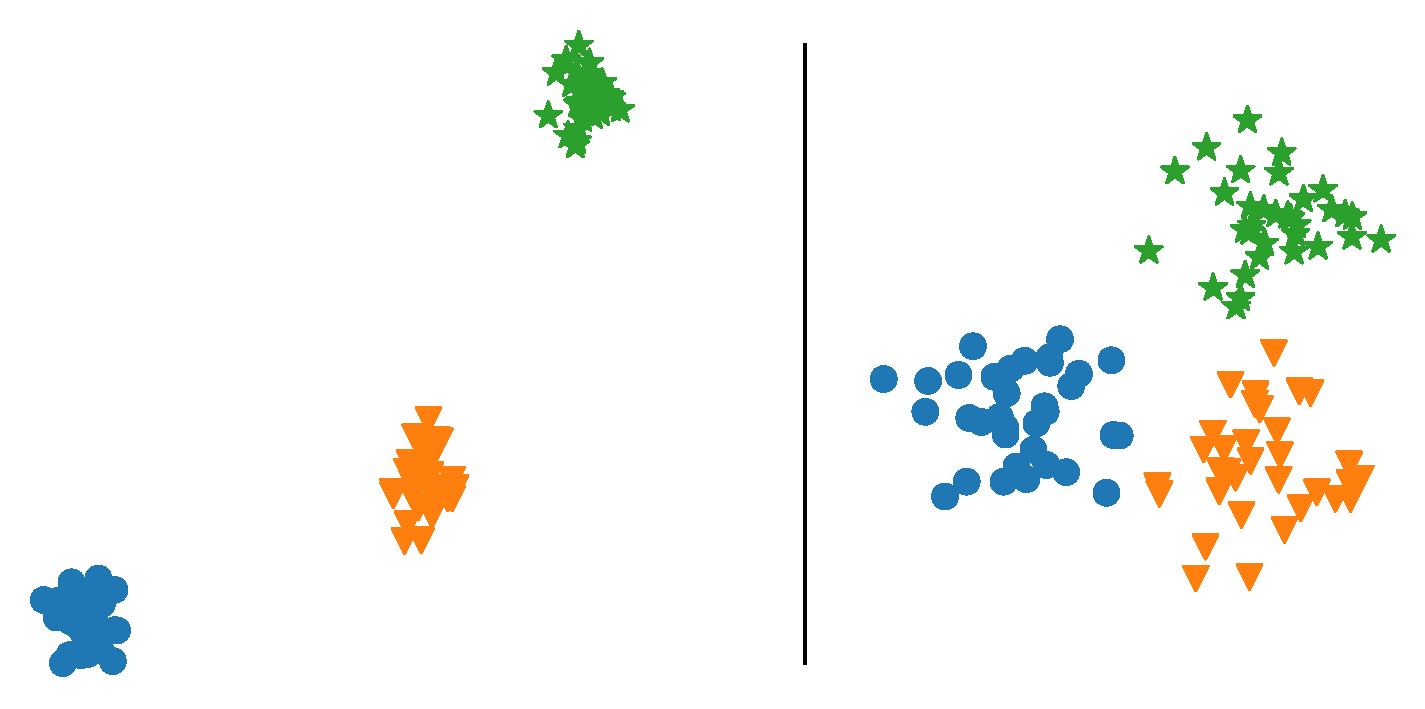
\includegraphics[width=0.5\textwidth]{figures/separability}
  \end{center}
\begin{itemize}
  \item Separability of clusters $k$ and $l$:
  \begin{equation*}
  s_{kl} = d(\muvec_k, \muvec_l)
  \end{equation*}
  \item Separability of a clustering:
  \begin{equation*}
  S = \frac{2}{K(K-1)}\sum_{k=1}^{K-1}\sum_{l=k+1}^{K}s_{kl}
  \end{equation*}
\end{itemize}
\end{frame}

\begin{frame}
\frametitle{1.1 Geometric Criteria}
\begin{itemize}
  \item \textbf{Silhouette coefficient.} First define $a(\xvec)$ as the mean distance between $\xvec$ and the other points in the cluster $k(\xvec)$ to which $\xvec$ is assigned:
  \begin{equation*}
  a(\xvec) = \frac{1}{|\cset_{k(\xvec)}| - 1} \sum_{\uvec \in \cset_{k(\xvec)}} d(\xvec, \uvec)
  \end{equation*}
  \item The quantity $b(\xvec)$ is defined as the smallest average distance between $\xvec$ and all points of another cluster $l \neq k(\xvec)$:
  \begin{equation*}
  b(\xvec) = \min_{l\neq k(\xvec)} \frac{1}{|\cset_l|} \sum_{\uvec \in \cset_l} d(\uvec, \xvec)
  \end{equation*}
\end{itemize}
\end{frame}

\begin{frame}
\frametitle{1.1 Geometric Criteria}
\begin{itemize}
  \item With $a$ and $b$ defined this way, we can define the silhouette coefficient for point $\xvec$:
  \begin{equation*}
  s(\xvec) = \frac{b(\xvec)-a(\xvec)}{\max{(b(\xvec), a(\xvec))}}
  \end{equation*}
  \item Finally, the \red{silhouette coefficient} for the whole clustering is:
  \begin{equation*}
  s = \frac1n \sum_{i=1}^{n} s(\xvec^i)
  \end{equation*}
\end{itemize}
\end{frame}


\begin{frame}
  \frametitle{1.2 Comparison between two partitions}
  \begin{itemize}
  \item We might want to compare a clustering $k$ to a ground truth. We assume that the $k(\xvec_i)$ is the cluster of sample $\xvec_i$ and $y_i$ the ground truth. 
  \item Difficulty: cluster labels are arbitrary.
  \item \red{Rand Index (RI):} percentage of pairs of points that are either in the same cluster in both partitions, or in different clusters in both partitions:
    \begin{equation*}
      \text{RI} = \frac2{n (n-1)} \sum_{i=1}^n \sum_{l=i+1}^n 
      \indic_{k(\xvec^i) = k(\xvec^l)} \, \indic_{y^i = y^l} + 
      \indic_{k(\xvec^i) \neq k(\xvec^l)} \, \indic_{y^i \neq y^l}.
    \end{equation*}
  \item Problem with RI: two random partitions can have a high RI by chance.
  \item Solution: ARI (Adjusted Rand Index) is the corrected version of RI.
  \item The same strategy can be applied to compare two clustering algorithms. 
  \end{itemize}
\end{frame}

% \begin{frame}
%   \frametitle{1.3 Cluster Stability}
%     \begin{center}
%       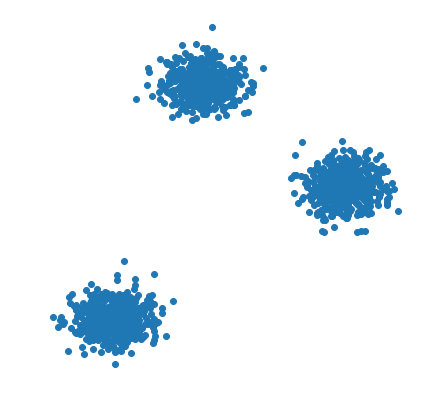
\includegraphics[width=0.7\textwidth]{figures/three_clusters}
%     \end{center}
% \end{frame}

\begin{frame}
  \frametitle{1.3 Cluster Stability}
  \begin{itemize}
    \item Generate several partitions with the same clustering algorithm while varying:
    \begin{itemize}
      \item the algorithm’s initialization
      \item sub-samplings of $\dset$
      \item (optionally) subsets of features
    \end{itemize}
    \item Compare the agreement between the different runs.
    \item A good clustering should reach a good agreement between different runs. 
  \end{itemize}
\end{frame}

\begin{frame}
  \begin{center}
    \large{2. Hierarchical Clustering}
  \end{center}
\end{frame}

% \begin{frame}
%   \frametitle{Dendrogram}
%   \begin{center}
%     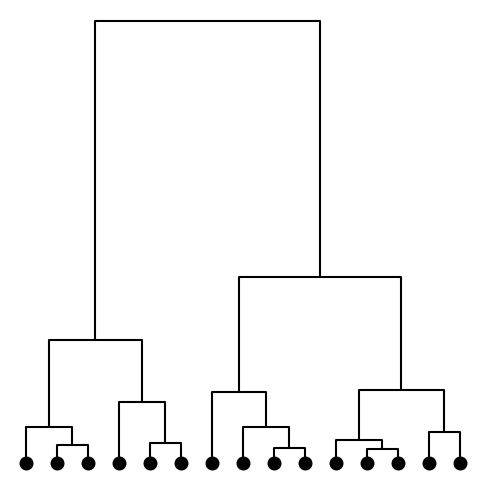
\includegraphics[width=0.7\textwidth]{figures/dendrogram}
%   \end{center}
% \end{frame}

\begin{frame}
  \frametitle{Construction}
  \begin{itemize}
  \item \red{Agglomerative} construction \textcolor{gray!70}{(bottom-up)}
    \begin{itemize}
    \item Initially: each point is its own cluster
    \item Iteratively merge the two closest clusters
    \end{itemize}
  \item \red{Divisive} construction \textcolor{gray!70}{(top-down)}
    \begin{itemize}
    \item Initially: all points belong to the same cluster
    \item Iteratively split clusters into two
    \end{itemize}
  \end{itemize}
\end{frame}

\begin{frame}
  \frametitle{Hierarchical Clustering - Principle}
  \begin{center}
    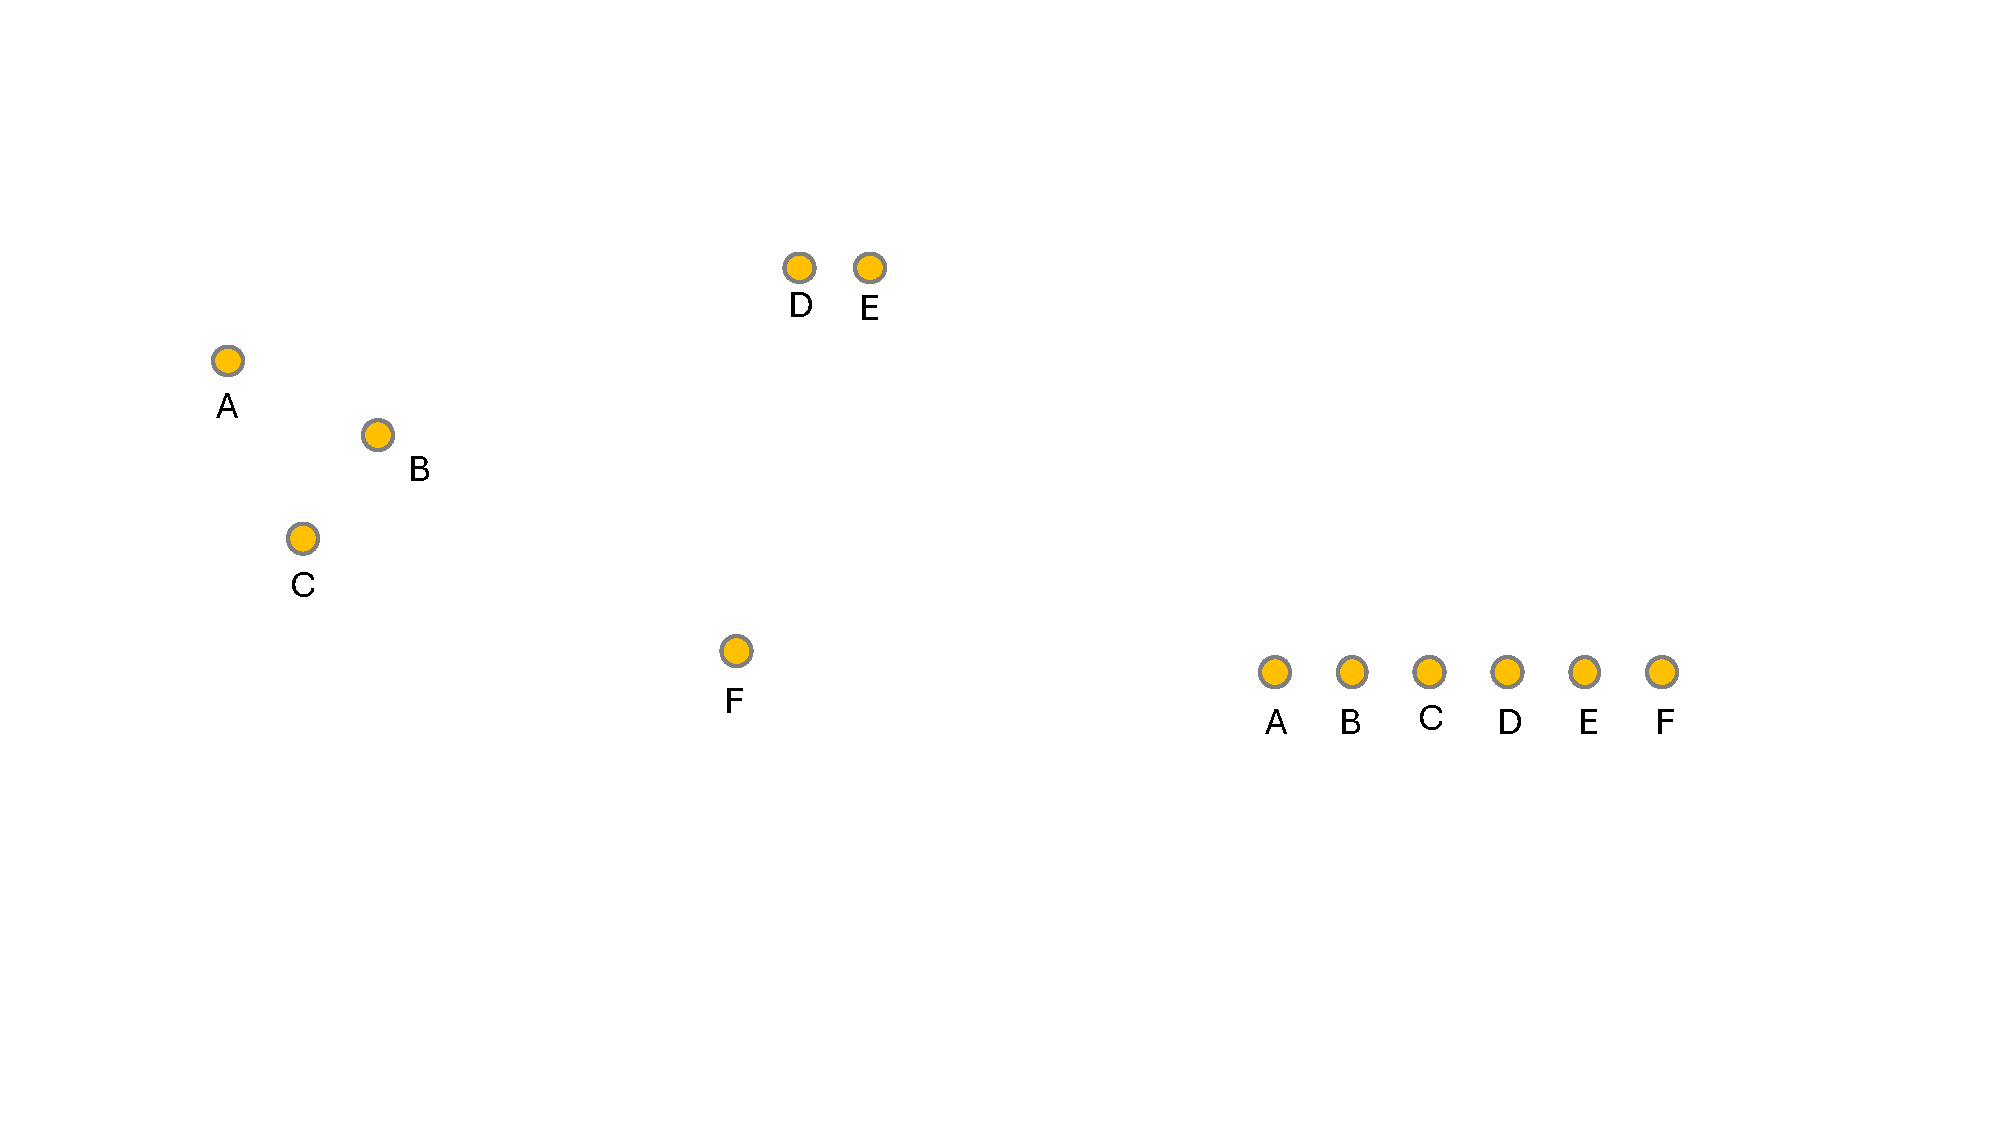
\includegraphics[width=0.8\textwidth]{figures/ch1}
  \end{center}
  Initialization: each point is its own cluster
\end{frame}

\begin{frame}
  \frametitle{Hierarchical Clustering - Principle}
  \begin{center}
    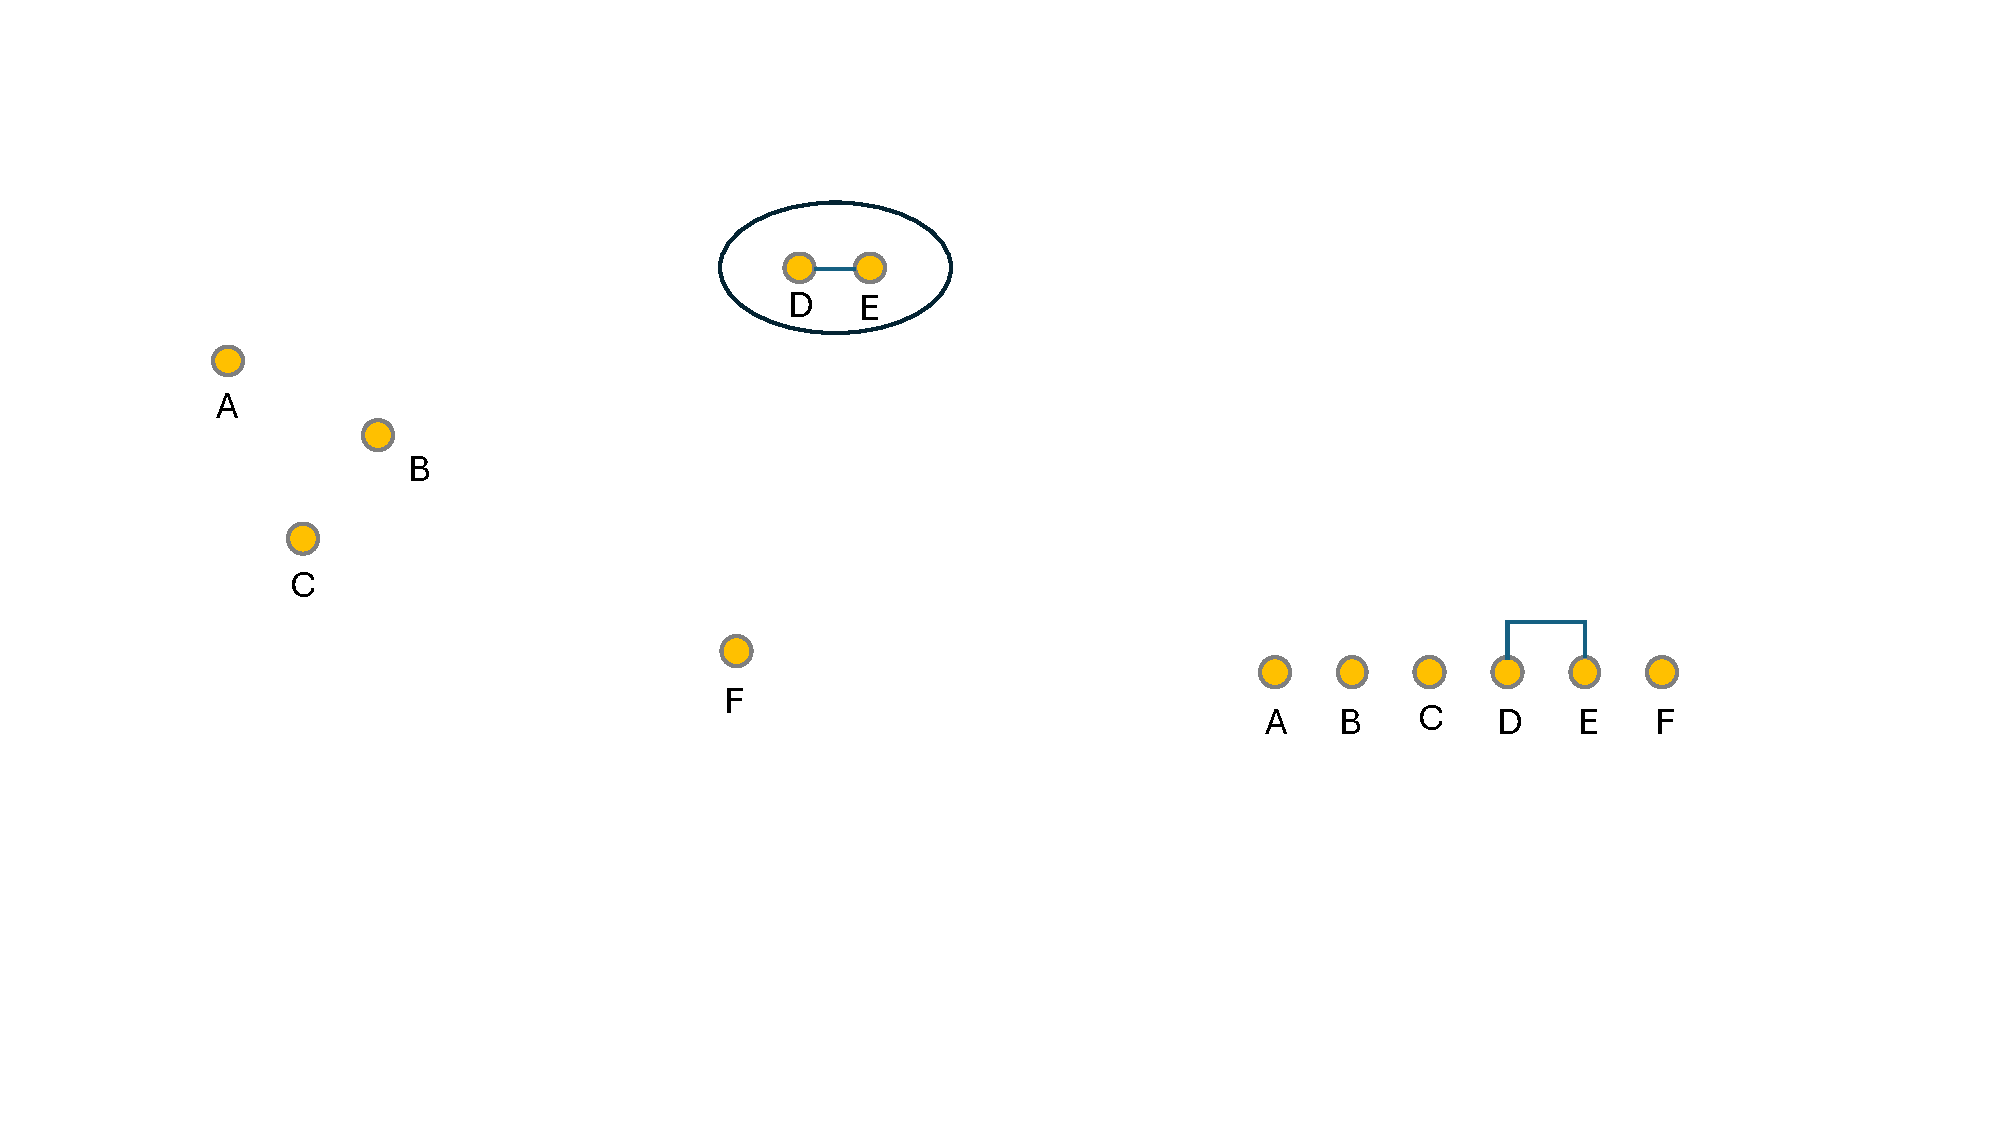
\includegraphics[width=0.8\textwidth]{figures/ch2}
  \end{center}
  The two closest points are merged and form the first cluster.
\end{frame}

\begin{frame}
  \frametitle{Hierarchical Clustering - Principle}
  \begin{center}
    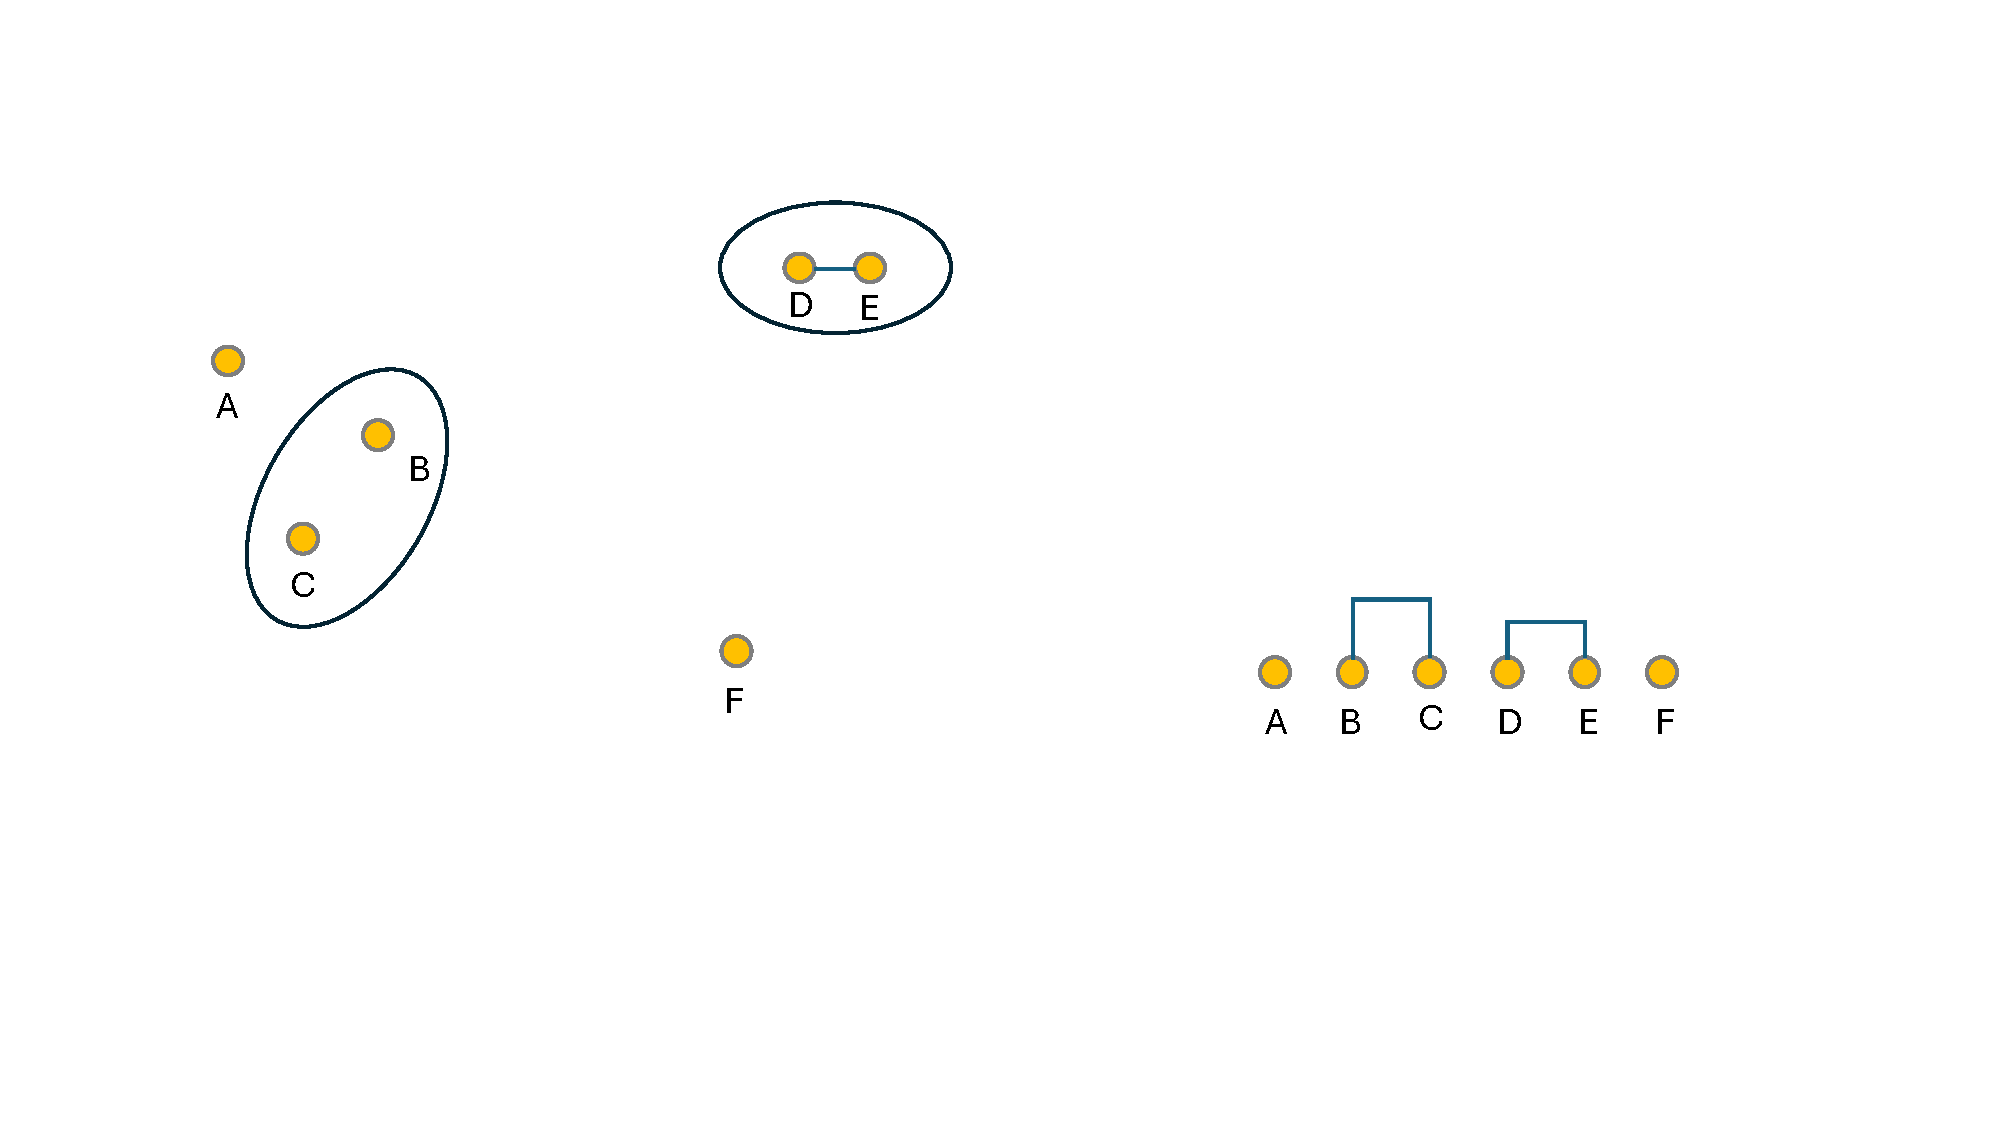
\includegraphics[width=0.8\textwidth]{figures/ch3}
  \end{center}
  Subsequently, the closest points (or clusters) are merged and form a new cluster.
\end{frame}

\begin{frame}
  \frametitle{Hierarchical Clustering - Principle}
  \begin{center}
    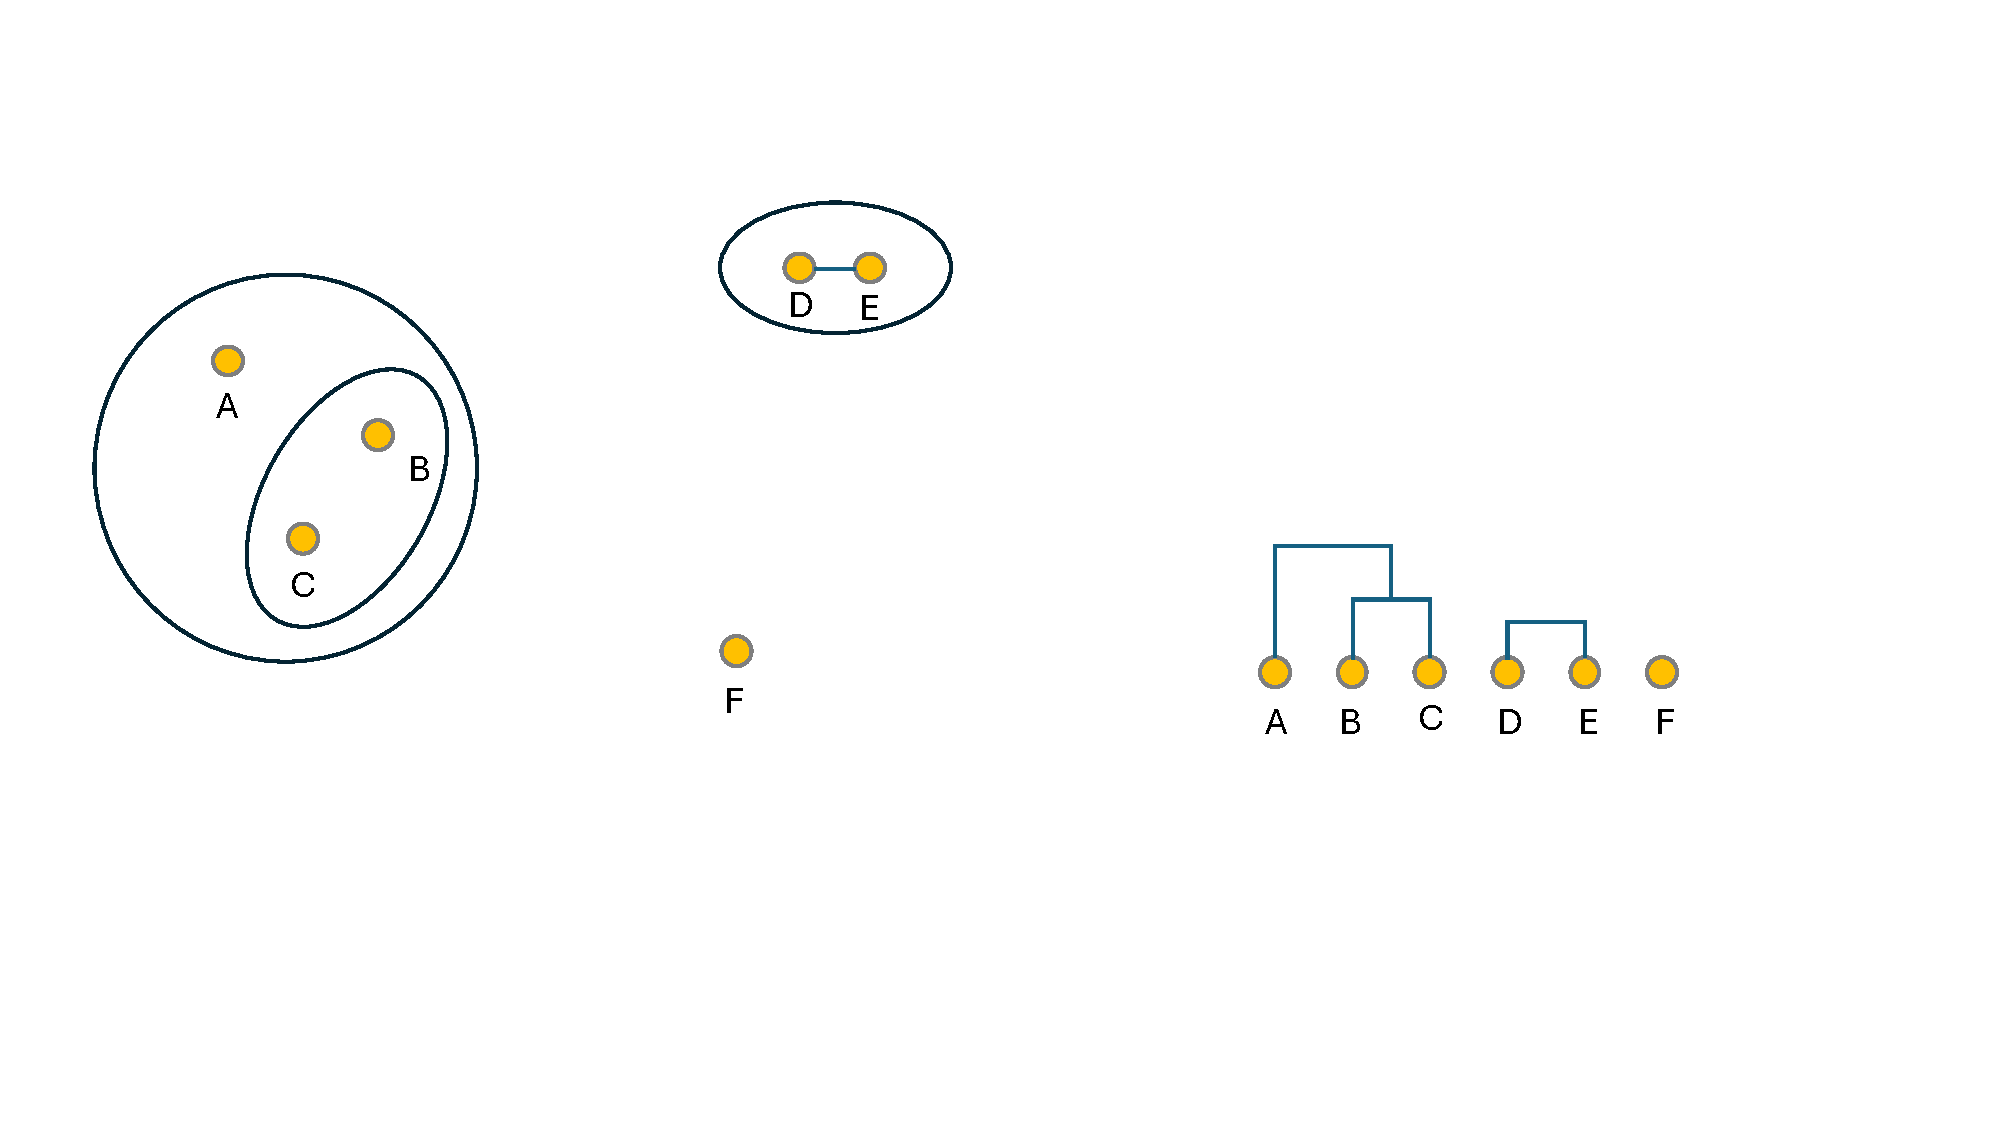
\includegraphics[width=0.8\textwidth]{figures/ch4}
  \end{center}
  A dendrogram is generated and keeps track of the fusion processes.
\end{frame}

\begin{frame}
  \frametitle{Hierarchical Clustering - Principle}
  \begin{center}
    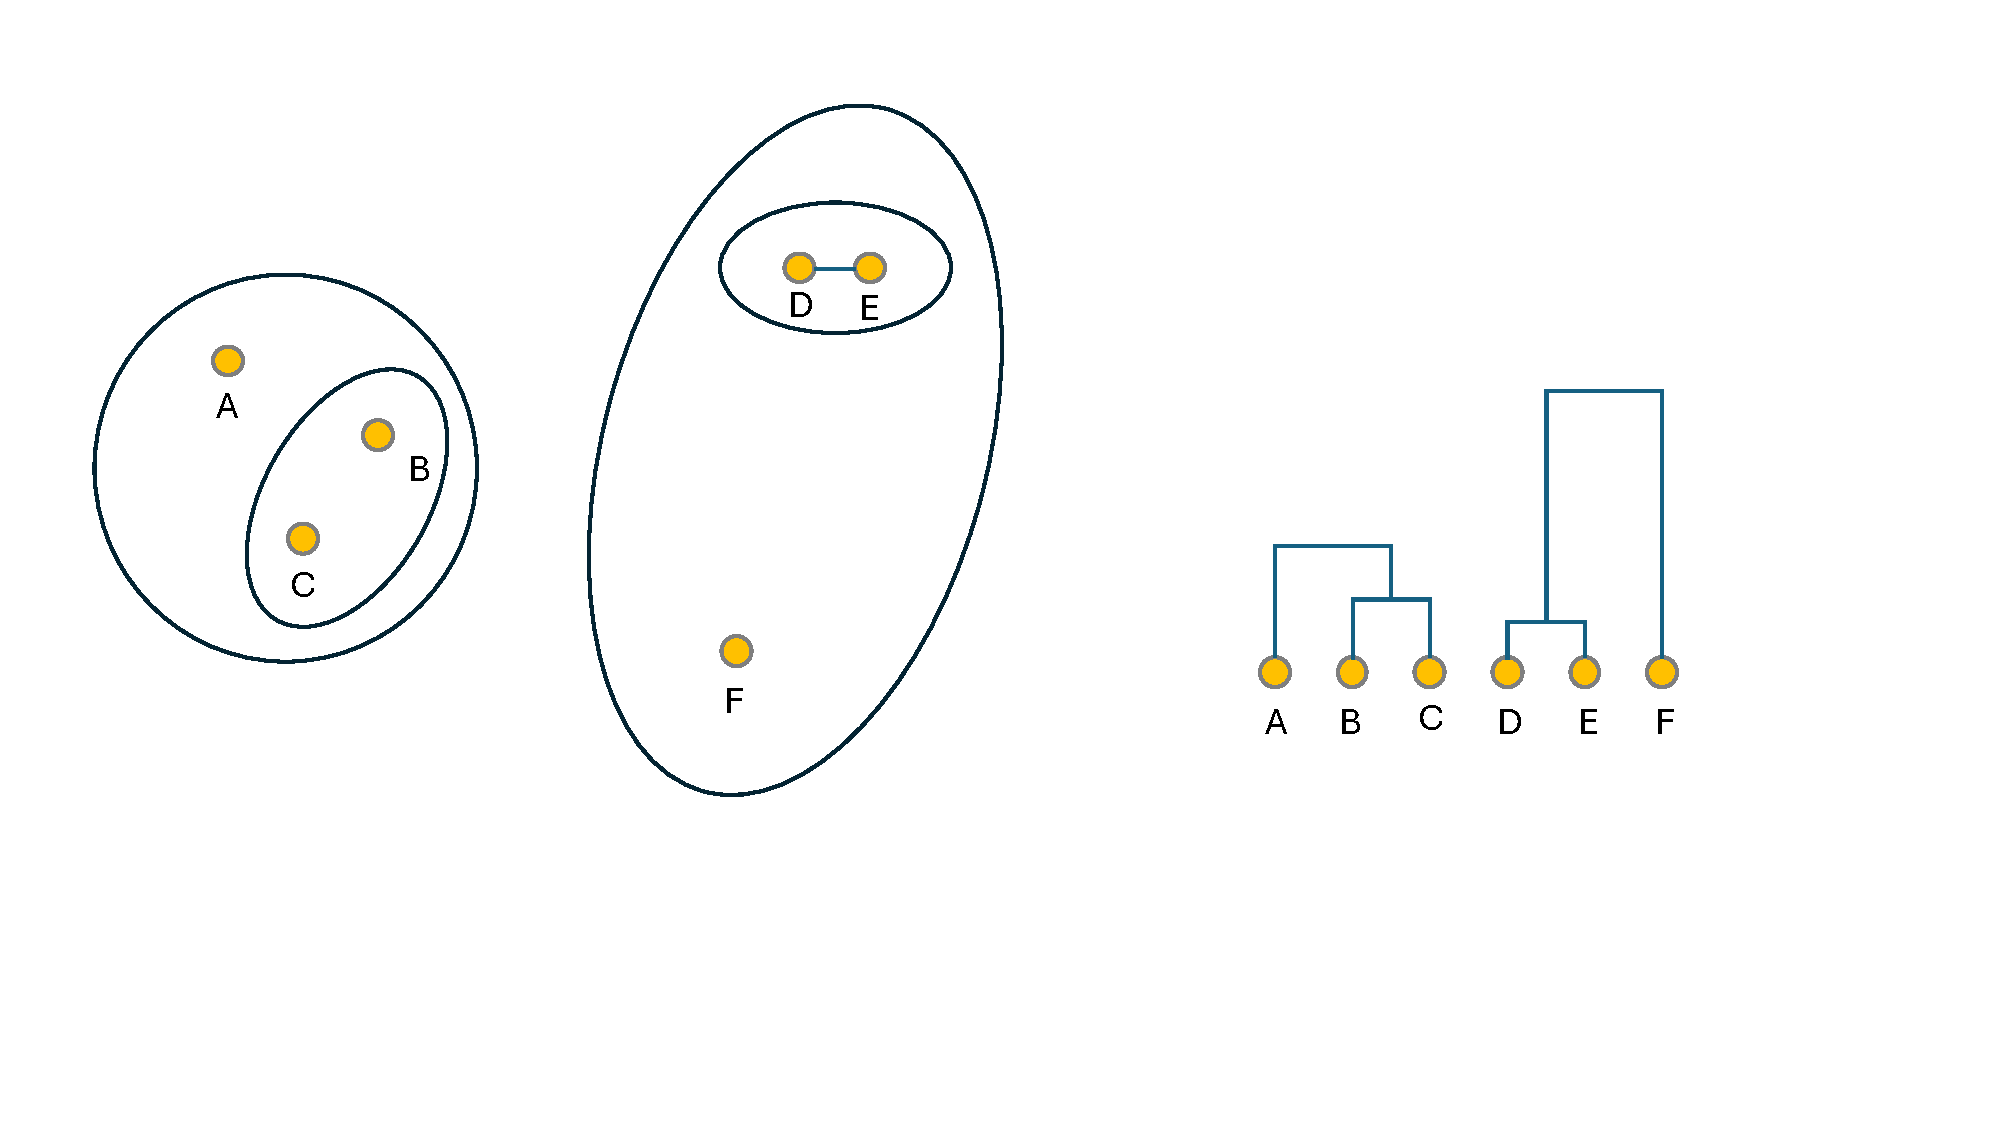
\includegraphics[width=0.8\textwidth]{figures/ch5}
  \end{center}
  The height of each fusion corresponds to the distance at which the fusion takes place.
\end{frame}



\begin{frame}
  \frametitle{Hierarchical Clustering - Principle}
  \begin{center}
    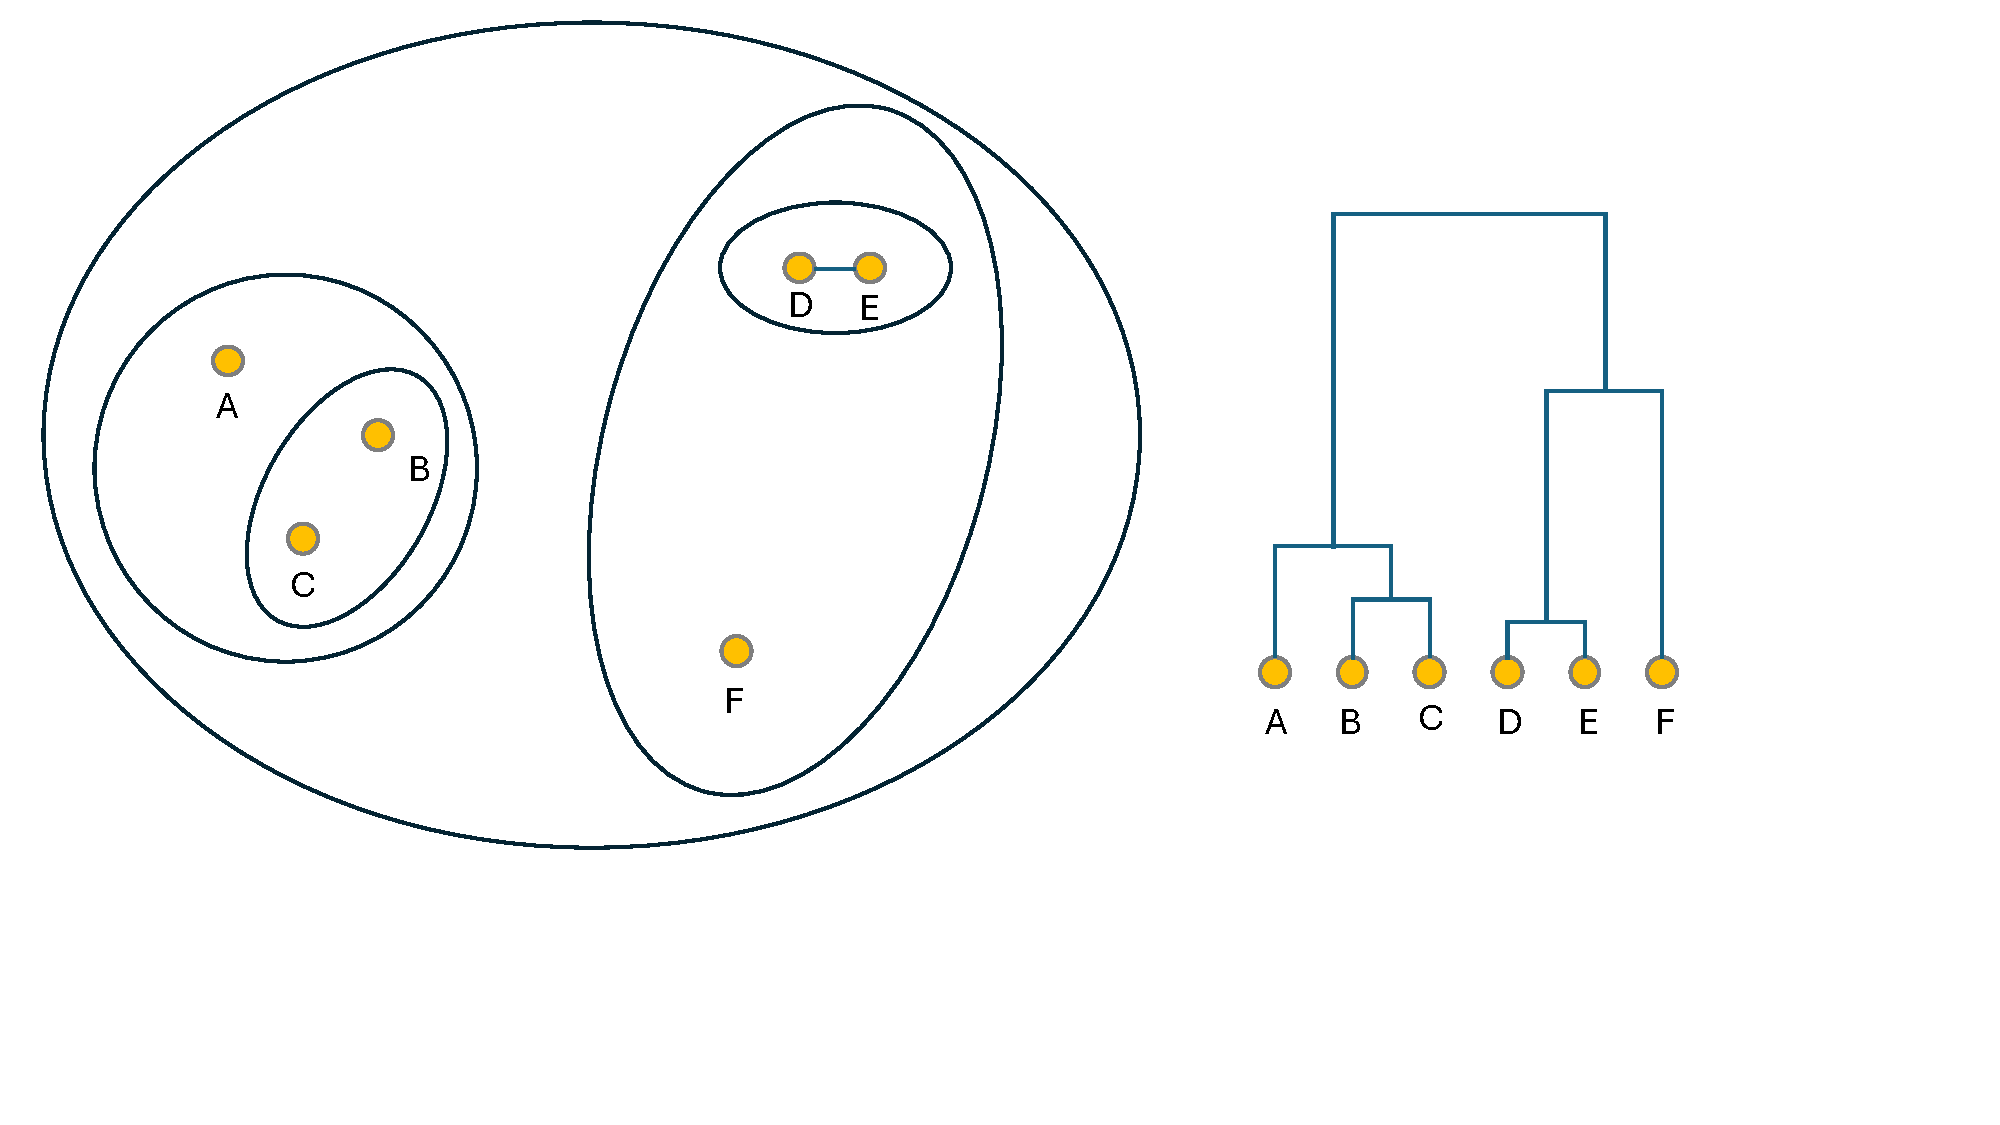
\includegraphics[width=0.8\textwidth]{figures/ch6}
  \end{center}
  The clustering stops when all points are in one global cluster. 
\end{frame}


\begin{frame}
  \frametitle{Hierarchical Clustering - 2 ingredients}
  \begin{itemize}
    \item Distance between points: 
    \begin{itemize}
      \item Recall: Each sample $\xvec_i$ corresponds to a point in feature space
      \item How do we calculate the distance between two points (samples)? 
    \end{itemize}
    \item Distance between clusters:
    \begin{itemize}
      \item Option 1 : represent each cluster by a prototype and calculate the point distance 
      \item Option 2 : calculate an aggregation of inter-point distances. 
    \end{itemize}
  \end{itemize}
\end{frame}

\begin{frame}{Hierarchical clustering: distances between points}
\begin{itemize}
  \item Here we assume two points $\xvec$ and $\yvec$; indices refer to the vector components
    \item \textbf{Euclidean distance} $d(\xvec,\yvec) = \sqrt{\sum_i (\xvec_i-\yvec_i)^2}$
    \item \textbf{Manhattan distance} $d(\xvec,\yvec) = \sum_i |\xvec_i-\yvec_i|$    
    \item \textbf{Cosine distance} $d(\xvec,\yvec) = 1 - \frac{\xvec^\top \yvec}{\|\xvec\|\|\yvec\|}$
    \item \textbf{Correlation distance} $d(\xvec,\yvec) = 1 - \mathrm{corr}(\xvec,\yvec)$
%    \item \textbf{Mahalanobis distance} $d(\xvec,\yvec) = \sqrt{(x-y)^\top \Sigma^{-1}(x-y)}$
\end{itemize}
\end{frame}



\begin{frame}
  \frametitle{Linkage Functions}
  \begin{itemize}
  \item \red{Linkage function:} distance between two clusters
    \begin{itemize}
    \item \red{Single linkage}
      \[ d_{\text{single}}(\cset_k, \cset_l) = \min_{(\uvec, \vvec) \in \cset_k \times \cset_l } d(\uvec, \vvec).
      \]
      \pause
    \item \red{Complete linkage}
      \[
        d_{\text{complete}}(\cset_k, \cset_l) = \max_{(\uvec, \vvec) \in \cset_k \times \cset_l} d(\uvec, \vvec).
      \]
      \pause
    \item \red{Average linkage} or UPGMA \textcolor{gray!70}{(Unweighted Pair Group Method with Arithmetic mean)}
      \[
        d_{\text{average}}(\cset_k, \cset_l) = \frac1{\lvert \cset_k \rvert} 
        \frac1{\lvert \cset_l \rvert}
        \sum_{\uvec \in \cset_k}\sum_{\vvec \in \cset_l} d(\uvec, \vvec).
      \]
    \end{itemize}
  \end{itemize}
\end{frame}

\begin{frame}[t]
  \frametitle{Linkage Functions}
  \begin{itemize}
  \item \red{Linkage function:} distance between two clusters
    \begin{itemize}
    \item \red{Centroid linkage}
      \[
        d_{\text{centroid}}(\cset_k, \cset_l) = d \left (\frac1{\lvert \cset_k \rvert} 
          \sum_{\uvec \in \cset_k} \uvec, 
          \frac1{\lvert \cset_l \rvert} \sum_{\vvec \in \cset_l} \vvec \right) = 
        d(\muvec_k, \muvec_l).
      \]
    \end{itemize}
  \end{itemize}
\end{frame}

\begin{frame}
  \begin{center}
    \large{3. k-Means Algorithm}
  \end{center}
\end{frame}

\begin{frame}
  \frametitle{Within-Cluster Variance}
  \begin{itemize}
  \item \red{Within-cluster variance}
    \[
            \text{Var}_\text{in}(\cset) = \frac1{\lvert \cset \rvert} \sum_{\xvec \in \cset}
      \ltwonorm{\xvec - \muvec}^2.
    \]
  \item Minimizing the within-cluster variance \(\Rightarrow\) create \blue{homogeneous} clusters
  \end{itemize}
\end{frame}

\begin{frame}
  \frametitle{Lloyd’s Algorithm}
  \begin{itemize}
  \item \blue{Initialization:} choose $\muvec_1, \muvec_2, \ldots, \muvec_K$ among the data points. 
  \item \blue{Assign} each observation $\xvec \in \dset$ to the nearest centroid:
    \begin{equation*}
      k(\xvec^i) = \argmin_{k=1, \ldots, K}\ltwonorm{\xvec^i - \muvec_k}^2
    \end{equation*}
  \item \blue{Recompute} the centroids $\muvec_k$. 
  \item \blue{Repeat} until the assignments no longer change. 
  \end{itemize}
\end{frame}

\begin{frame}
  \frametitle{Lloyd’s Algorithm}
  \begin{itemize}
  \item \blue{Advantages:}
    \begin{itemize}
    \item Converges quickly in practice
    \end{itemize}
    \pause
  \item \blue{Limitations:}
    \begin{itemize}
    \item Requires the number of clusters $K$ to be specified in advance
    \item \blue{Greedy} approach — no guarantee of reaching the global minimum
    \item \blue{Stochasticity:} results depend on initialization
    \item Clusters are necessarily \blue{convex}
    \end{itemize}
  \end{itemize}
\end{frame}

\begin{frame}
  \begin{center}
    \large{4. DBSCAN}
  \end{center}
\end{frame}

\begin{frame}
  \frametitle{DBSCAN: Motivation}
  \begin{center}
    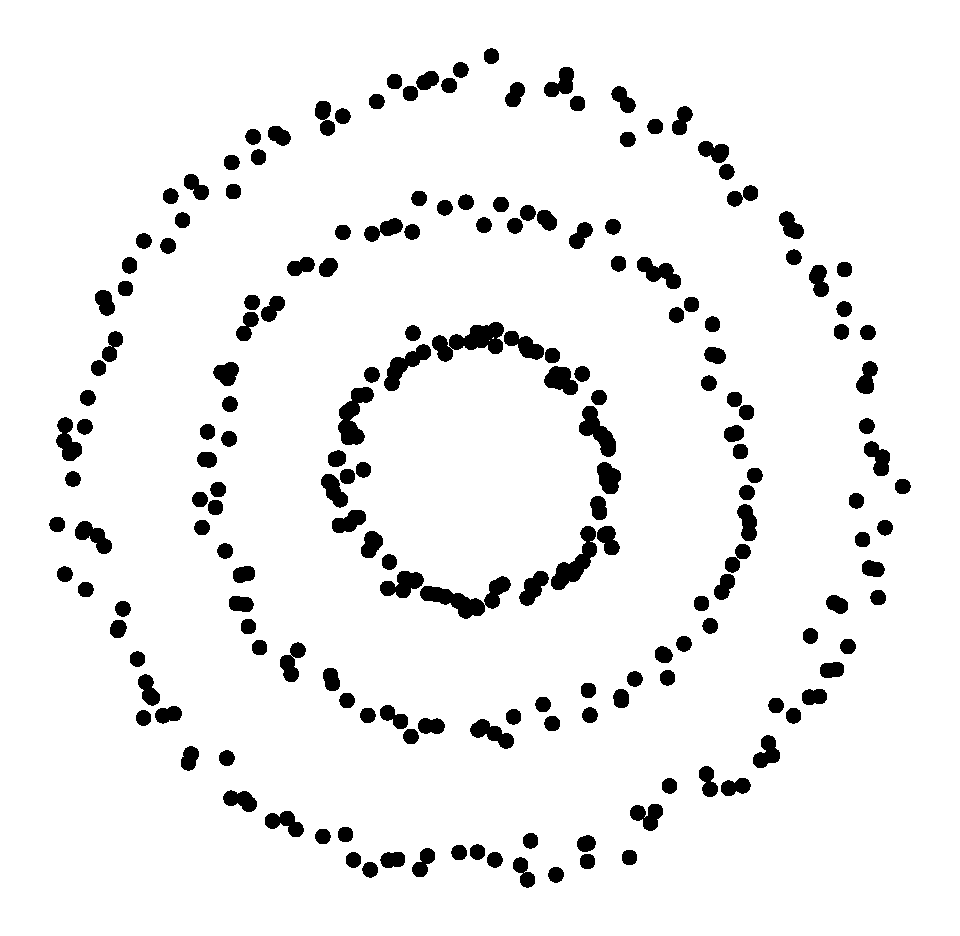
\includegraphics[width=.3\textwidth]{figures/dbscan_pb}%
    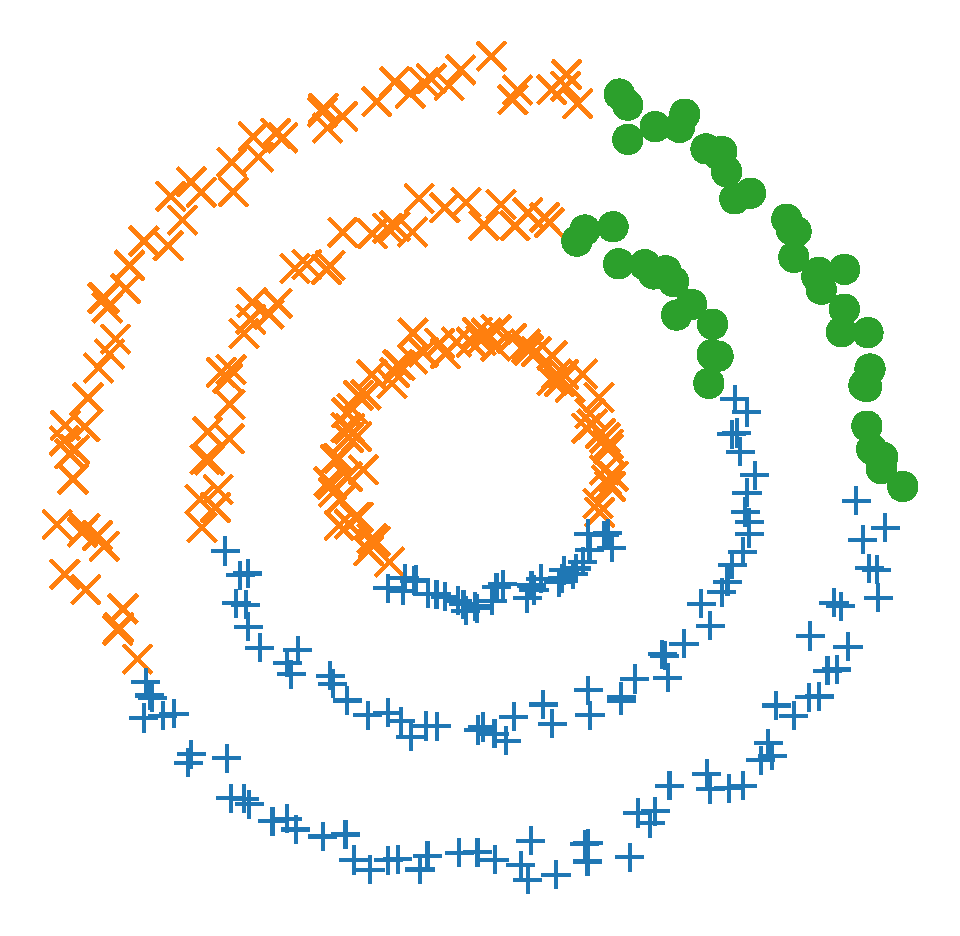
\includegraphics[width=.3\textwidth]{figures/hierarchical_sol}% 
    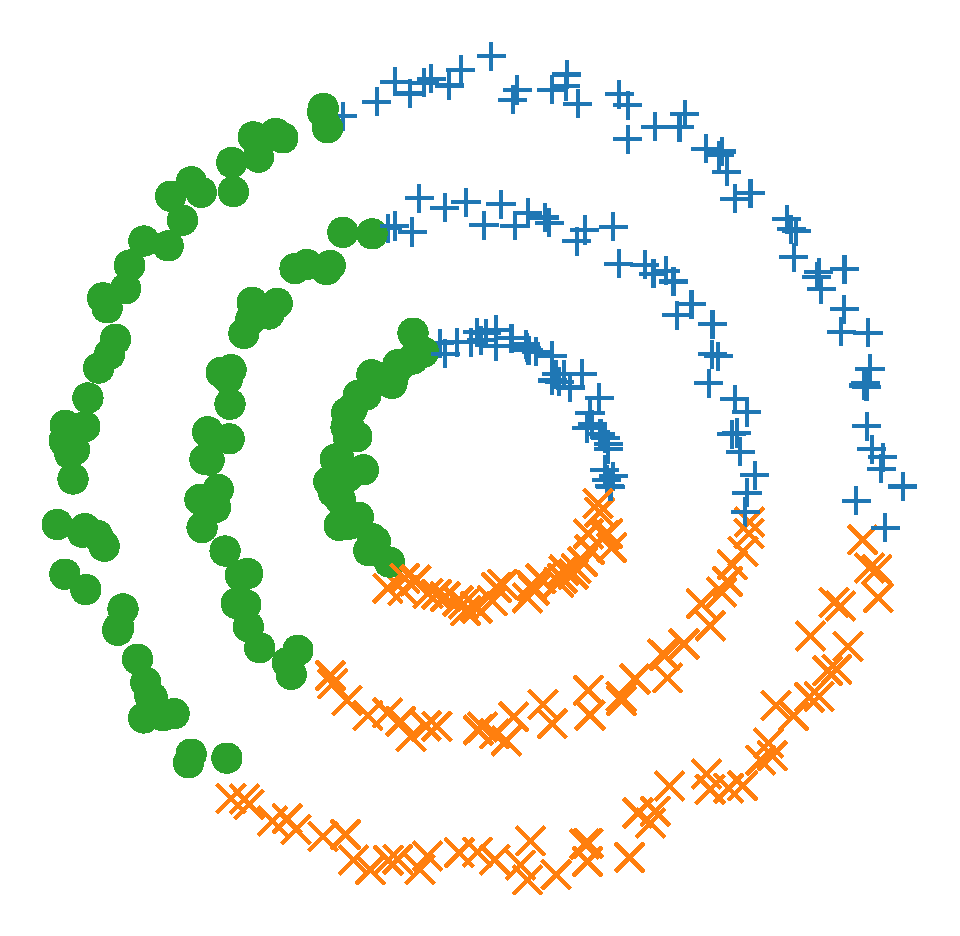
\includegraphics[width=.3\textwidth]{figures/kmeans_sol}
    
    {\small Point cloud – hierarchical clustering – k-means clustering}
  \end{center}
  \begin{itemize}
  \item Idea: use \blue{density}
  \end{itemize}
\end{frame}

\begin{frame}
  \frametitle{DBSCAN}
  \begin{itemize}
  \item Idea: iterate \blue{from neighbor to neighbor} using \blue{neighborhoods} (balls) of radius $\varepsilon$.
  \item Two parameters are defined:
  \begin{enumerate}
    \item a radius $\varepsilon$
    \item a minimum number of points $n_{min}$
  \end{enumerate}
  \item Definitions:
  \begin{itemize}
    \item \textbf{Core point:} a point having at least $n_{min}$ neighbors within a radius $\varepsilon$.
    \item \textbf{Border point:} has fewer than $n_{min}$ neighbors, but lies close to a core point.
    \item \textbf{Noise point (outlier):} isolated points, considered as noise.
  \end{itemize}
\end{itemize}
\end{frame}

\begin{frame}
  \frametitle{DBSCAN}
  \begin{itemize}
  \item Steps of the algorithm:
  \begin{itemize}
    \item Identify core points.
    \item Build connected components by linking neighboring core points — each component forms a cluster.
    \item Assign each border point to a connected component.
    \item Noise points remain unassigned.
  \end{itemize}
  \end{itemize}
  \begin{center}
    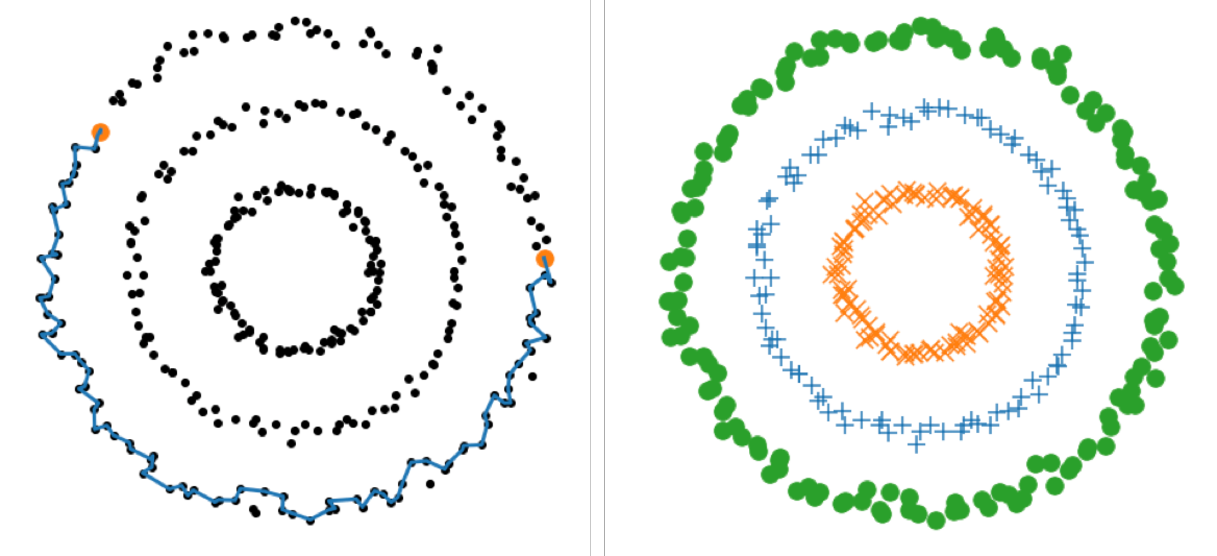
\includegraphics[width=.6\textwidth]{figures/dbscan}
  \end{center}
\end{frame}

\begin{frame}
  \frametitle{DBSCAN: Advantages and Limitations}
  \begin{itemize}
  \item \blue{Advantages:}
    \begin{itemize}
    \item No assumption about cluster shape
    \item Simple, no need to define the number of clusters
    \item Robust to outliers
    \end{itemize}
  \pause
  \item \blue{Limitations:}
    \begin{itemize}
    \item Does not handle varying densities well
    \item Few theoretical guarantees
    \item Not applicable in very high-dimensional spaces
    \end{itemize}
  \end{itemize}
\end{frame}

\begin{frame}
  \frametitle{Clustering: conclusion}
  \begin{itemize}
    \item Clustering refers to the partitioning of a dataset $\{\xvec_i\}_{i=1..N}$ into groups. 
    \item There are many quality measures for clustering: 
    \begin{itemize}
      \item Geometric measurements and separability
      \item Robustness
      \item Comparison to partial ground truth. 
    \end{itemize}
    \item Algorithms: 
    \begin{itemize}
      \item Hierarchical clustering: good for exploration
      \item k-means: most popular method (but we need to fix the number of clusters)
      \item DBSCAN / HDBSCAN: widely used
    \end{itemize}
  \end{itemize}
\end{frame}

\begin{frame}
  \frametitle{Clustering: limitations}
  \begin{itemize}
    \item There is no general way to state whether a clustering "makes sense", other than some comparison (systematic or anecdotal) to ground truth.
    \item Correlation structure:
    \begin{itemize}
      \item Strongly correlated data will dominate distances: $d(\xvec, \yvec) = \sqrt{\sum_i(x_i -  y_i)^2}$
      \item Using PCA to decorrelate does not solve this issue, unless PCs are normalized with respect to their variance (whitening). But then, we also increase noise.
    \end{itemize}
    \item There is no real "unsupervised approach": 
    \begin{itemize}
      \item We choose features
      \item We choose methods, distances, hyperparameters
    \end{itemize}
  \end{itemize}
\end{frame}

\begin{frame}
  \frametitle{Clustering: an ill-posed problem}
  \begin{center}
    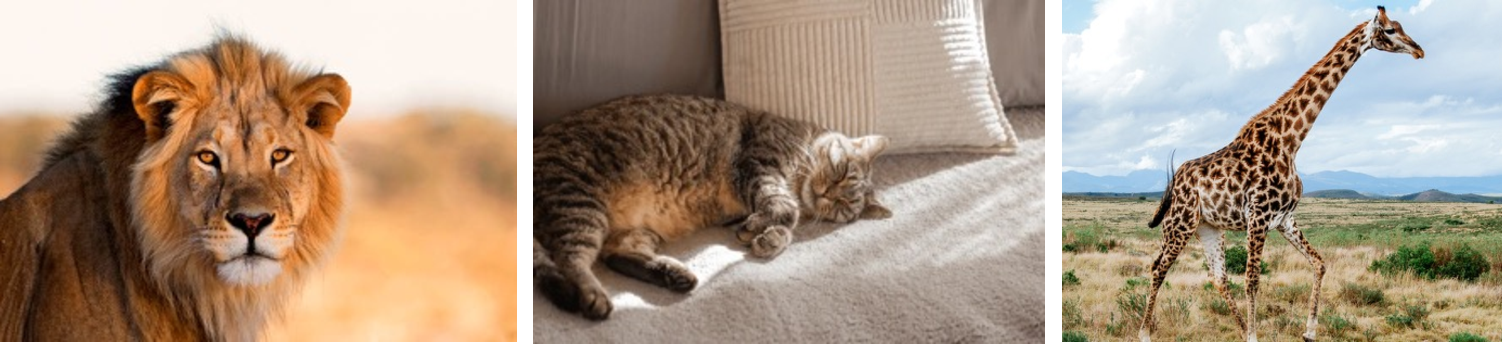
\includegraphics[width=0.9\textwidth]{figures/clustering_animals}
  \end{center}
  How to define two groups for these images? 
\end{frame}












